%----------------------------------------------------------------------------------------
%	PACKAGES AND OTHER DOCUMENT CONFIGURATIONS
%----------------------------------------------------------------------------------------

\documentclass[12pt]{article}
\usepackage{polski}
\usepackage[polish]{babel}
\usepackage[utf8]{inputenc}
\usepackage{datetime}
\usepackage{graphicx}
\usepackage{tikz}
\usepackage{amsmath}
\usepackage{multirow}
\usepackage{tabularx}
\usepackage{geometry}
\usepackage{subcaption}
\usepackage{epstopdf}
\usepackage{hyperref}
\usepackage{indentfirst}

\geometry{
 	a4paper, 
 	left    = 20mm,
 	right	  = 20mm,
 	top     = 20mm,
 	bottom  = 20mm,
}
 
%----------------------------------------------------------------------------------------
 
%----------------------------------------------------------------------------------------
% DATES
%----------------------------------------------------------------------------------------

\renewcommand{\dateseparator}{.}
\newdate{exercise_date}{15}{12}{2016}


% dodatkowe typy kolumn tabel

% flush left fixed width:
\newcolumntype{L}[1]{>{\raggedright\arraybackslash}p{#1}}

% center fixed width:
\newcolumntype{C}[1]{>{\centering\arraybackslash}p{#1}}

% flush right fixed width:
\newcolumntype{R}[1]{>{\raggedleft\arraybackslash}p{#1}}

%----------------------------------------------------------------------------------------

%----------------------------------------------------------------------------------------
% TIKZ PACKAGES
%----------------------------------------------------------------------------------------

\usetikzlibrary{arrows}

%----------------------------------------------------------------------------------------

\begin{document}
 
\begin{titlepage}

\newcommand{\HRule}{\rule{\linewidth}{0.5mm}}
% Defines a new command for the horizontal lines, change thickness here

\center
% Center everything on the page
 
%----------------------------------------------------------------------------------------
%	LOGO SECTION
%----------------------------------------------------------------------------------------


\includegraphics[width=6cm]{./img/logo.png}\\[1cm]
% Include a department/university logo - this will require the graphicx package
 
%----------------------------------------------------------------------------------------
 
%----------------------------------------------------------------------------------------
%	HEADING SECTIONS
%----------------------------------------------------------------------------------------

\textsc{\LARGE Akademia Górniczo-Hutnicza \\[0.2cm]
im. Stanisława Staszica w Krakowie}\\[1.5cm]
% Name of your university/college

\textsc{\Large Elektroniczne systemy diagnostyki medycznej i terapii}\\[0.5cm]
% Major heading such as course name

%----------------------------------------------------------------------------------------
%	TITLE SECTION
%----------------------------------------------------------------------------------------

\HRule \\[0.5cm]
{ \huge \bfseries Klasyfikacja pulsu - Naiwny Bayes}\\[0.3cm]
% Title of your document
\HRule \\[1.5cm]

\flushright
\Large \emph{Autorzy:}\\
Piotr \textsc{Janus}\\[0.1cm]  % Your name
Kamil \textsc{Piszczek}\\[3cm]        % Your name
% Authors

%----------------------------------------------------------------------------------------
%	DATE SECTION
%----------------------------------------------------------------------------------------
% Data wykonania ćwiczenia: \\
%{\large \displaydate{exercise_date}}\\[1cm]


\vfill % Fill the rest of the page with whitespace

\end{titlepage}
\section{Wstęp}
\label{sec_wstep}

Naiwny klasyfikator Bayesa jest prostym klasyfikatorem probabilistycznym opartym na twierdzeniu Bayesa. Jest nazywany naiwnym ze względu na przyjęte założenie, mówiące, że poszczególne cechy są wzajemnie niezależne. Pomimo tak dużego uproszczenia, klasyfikator wypada niespodziewanie dobrze w wielu rzeczywistych problemach. Jego dużą zaletą jest dobra skalowalność, operuje on jedynie na jawnych wzorach w przeciwieństwie do innych metod wykorzystujących podejście iteracyjne.

Jednym z zastosowań klasyfikatora jest diagnozowanie wad i dysfunkcji serca na podstawie sygnału EKG, a dokładniej występującego w nim zespołu QRS. Jest to zespół opisujący pobudzenie mięśni serca. Uproszczony przebieg EKG z zespołem QRS został umieszczony na rysunku \ref{fig_qrs}.

\begin{figure}[!htb]
  \begin{center}
    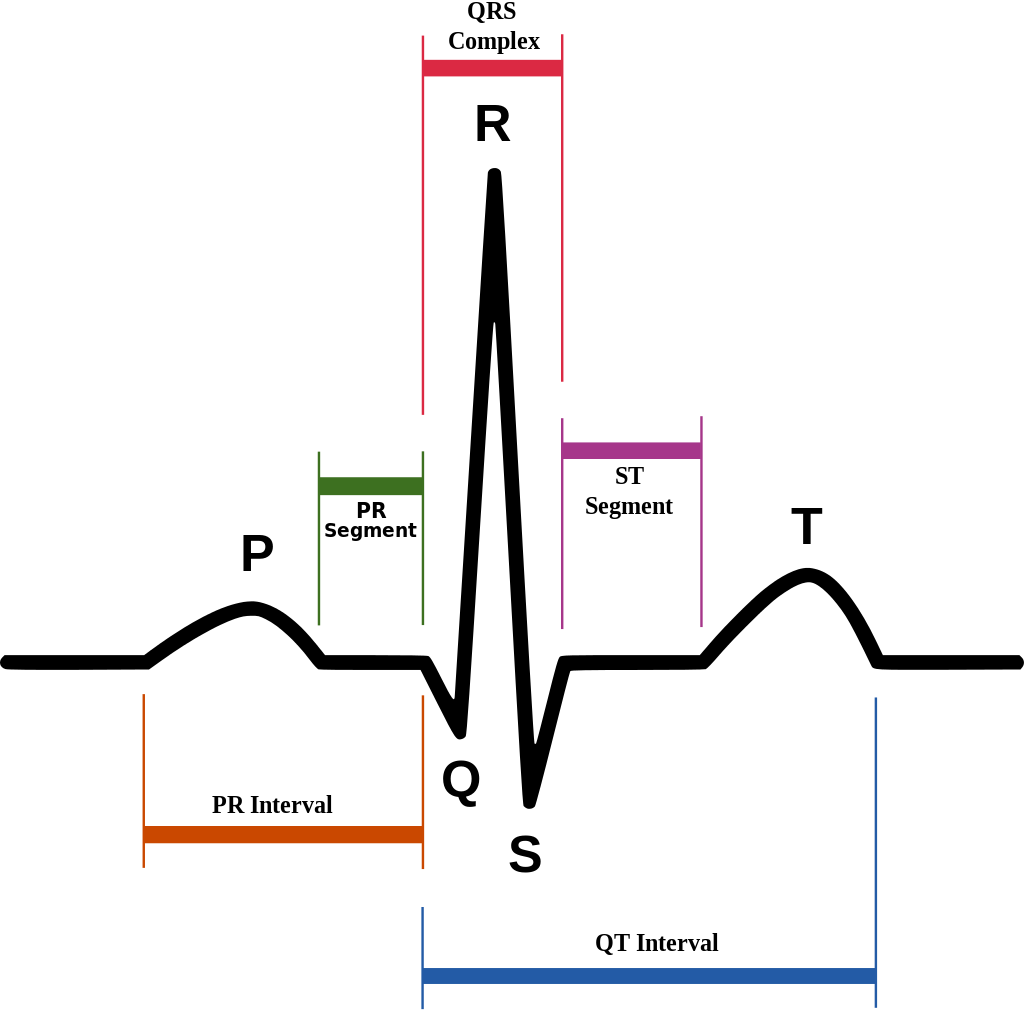
\includegraphics[scale = 0.25]
    {img/qrs.png}
  \end{center}
  \caption{Uproszczony zespół QRS -- źródło \cite{bibWikipedia}}
  \label{fig_qrs}
\end{figure}

W celu dokonania klasyfikacje konieczne jest zdefiniowanie wskaźników opisujących QRS. Na podstawie rysunku \ref{fig_qrs} możemy wyróżnić następujący cechy:

	\begin{itemize}
	\item{Wartość szczytowa załamka R i moment jej wystąpienie} 
	\item{Odstęp pomiędzy wcześniejszym a obecnie analizowanym załamkiem R}
	\item{Odstęp pomiędzy aktualnie analizowanym i kolejnym załamkiem R}
	\item{Początek/koniec oraz początkowa/końcowa wartość załamka P}
	\item{Wartość szczytowa załamka P i moment jej wystąpienia}
	\item{Początek/koniec i wartość początkowa/końcowa całego zespołu QRS}
	\item{Wartość szczytowa załamka T i moment jego wystąpienia}
	\item{Koniec i wartość końcowa załamka T}
	\end{itemize}
\section{Algorytm}
\label{sec_algorytm}

\subsection{Założenia}
\label{subsec_zalozenia}

Idee metody Naiwnego Bayesa można łatwo wyjaśnić na prostym przykładzie, precyzyjny opis matematyczny został zamieszczony w rozdziale \ref{sec_opis_mat}. Na rysunku \ref{fig_bayes_przyklad} przedstawiony został zbiór punktów, podzielony na dwie klasy (czerwone i zielone). Zadaniem klasyfikatora jest przydzielenie nowego obiektu do jednej z tych klas. W tym przypadku klasyfikacja będzie dokonana na podstawie położenia i elementów znajdujących się w sąsiedztwie nowo dodanego obiektu. Podany zbiór punktów, pełni w tym przypadku rolę zbioru uczącego.

\begin{figure}[!htb]
  \begin{center}
    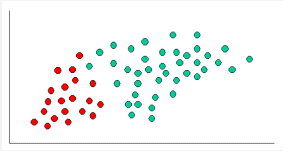
\includegraphics[scale = 1]
    {img/bayes_przyklad.png}
  \end{center}
  \caption{Prosty przykład - zbiór punktów (źródło \ref{})}
  \label{fig_bayes_przyklad}
\end{figure}

\subsection{Klasyfikacja}
\label{subsec_klasyfikacja}

W omawianym przykładzie możemy zauważyć, że obiektów zielonych jest dwa razy więcej niż czerwonych. W związku z tym możemy założyć ''z góry'', że nowy obiekt ma dwa razy większe prawdopodobieństwo bycia zielonym niż czerwonym. Obliczone w ten sposób prawdopodobieństwo nazywane jest prawdopodobieństwem \textit{a priori}. 

Wszystkich obiektów jest 60 w czym 40 zielonych i 20 czerwonych. Prawdopodobieństwo \textit{a priori} wylicza się jako iloraz liczby obiektów danego koloru do liczby wszystkich obiektów. Następnie przystępujemy do kolejnego etapu klasyfikacji, przyjmijmy pewne sąsiedztwo nowego punktu (rysunek \ref{fig_bayes_przyklad2}). Możemy założyć, że im więcej obiektów danego koloru w otoczeniu nowego obiektu, tym bardziej prawdopodobne, że jest on tego koloru. Wyznaczone w ten sposób prawdopodobieństwo nazywane jest szansą, oblicza się je jako stosunek liczby obiektów danego koloru w sąsiedztwie, do całkowitej liczby obiektów tego koloru.

\begin{figure}[!htb]
  \begin{center}
    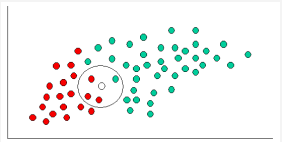
\includegraphics[scale = 1]
    {img/bayes_przyklad_2.png}
  \end{center}
  \caption{Prosty przykład - sąsiedztwo (źródło \ref{})}
  \label{fig_bayes_przyklad2}
\end{figure}

Mając dane prawdopodobieństwo \textit{a priori} oraz szansę, możemy przystąpić do ostatniego etapu klasyfikacji. Końcowe prawdopodobieństwo czy nowy obiekt należy do danej klasy (jest danego koloru) obliczane jest jako iloczyn dwóch wyznaczonych wcześniej prawdopodobieństw. Zostaje on oczywiście przypisany do klasy o większym prawdopodobieństwie.


\subsection{Wykorzystanie w detekcji pulsu}
\label{subsec_bayes_detekcja_pulsu}

Omówiony w poprzednich punktach przykład, był bardzo uproszczony i miał na celu jedynie pokazać idee klasyfikatora. Klasyfikacja zespołu QRS jest problemem wielowymiarowym (dokładnie 18 wymiarowym, gdyż jest to rozmiar wektora cech). W takim przypadku nieco inaczej oblicza ''szansa''. Obliczane jest osobno prawdopodobieństwo przynależności do danej klasy na podstawie każdego elementu z wektora cech. Ostatecznie pod uwagę brany jest iloczyn wszystkich prawdopodobieństw.

Kolejnym zagadnieniem jest sposób obliczania prawdopodobieństwa na podstawie cechy. W przypadku niniejszego projektu wykorzystywany jest w tym celu rozkład normalny (rozdział \ref{sec_rozklady}). Dla każdej klasy, poszczególne cechy mają przypisaną wartość średnią i odchylenie standardowe. Są one obliczane na podstawie zbioru uczącego w trakcie procesu uczenia.

\subsection{Zbiór testowy i uczący}
\label{subsec_test_ucz}


\section{Opis matematyczny}
\label{sec_opis_mat}

\subsection{Twierdzenie Bayesa}
\label{subsec_tw_bayesa}
Twierdzenie w teorii prawdopodobieństwa określające zależność między prawdopodobieństwem warunkowym wystąpienia zdarzeń $A|B$ i $B|A$. Przyjmijmy zbiór zdarzeń $X$, w którym zdarzenia $B_i \in X$, $P(B_i)>0$ ${(i=1,2, \dots , n)}$ tworzą układ zupełny (iloczyn każdych dwóch zdarzeń jest zdarzeniem niemożliwym, natomiast suma wszystkich zdarzeń jest zdarzeniem pewnym). Wówczas dla dowolnego $A \in X$ zachodzi następująca zależność:

	\begin{equation}
	\label{eq_tw_bayesa_1}
		P(B_i | A) = \frac{P(A | B_i) P(B_i)}{P(A)}
	\end{equation}

Wykorzystując dodatkowo wzór na prawdopodobieństwo całkowite, powyższa zależność może zostać przekształcona do następującej postaci:

	\begin{equation}
	\label{eq_tw_bayesa_2}
		P(B_i | A) = \frac{P(A | B_i) P(B_i)}{\sum_{k=1}^{n} P(A | B_k)P(B_k)}
	\end{equation}


\subsection{Model probabilistyczny}
\label{subsec_model}

Zdefiniujmy k-elementowy zbiór klas $C = {\{C_1, C_2, \dots, C_k\}}$ oraz dane do klasyfikacji opisane jako wektor ${x = \{x_1, x_2, \dots, x_n\}}$ zawierający $n$ niezależnych cech. Prawdopodobieństwo przynależności do danej klasy może zostać zapisane z wykorzystaniem twierdzenia Bayesa (rozdział \ref{subsec_tw_bayesa}):

	\begin{equation}
	\label{eq_p_ck_x}
		P(C_i | x) = \frac{P(x | C_i) P(C_i)}{P(x)}
	\end{equation}

Prawdopodobieństwo $P(x)$ występujące w mianowniku wzoru (\ref{eq_p_ck_x}) nie zależy od $C$ i jest stałe, licznik może natomiast zostać przekształcony poprzez wykorzystanie definicji prawdopodobieństwa warunkowego:

	\begin{equation}
	\label{eq_p_numerator1}
		P(x_1, \dots , x_n | C_i)P(C_i) = P(x_1, \dots, x_n, C_i)
	\end{equation}

	\begin{equation}
	\label{eq_p_numerator2}
		P(x_1, \dots, x_n, C_i) = P(x_1 | x_2 , \dots , x_n, C_i)P(x_2 | x_3, \dots , x_n, 	C_i) \dots P(x_{n-1} | x_n, C_i)P(x_n | C_i)P(C_i)
	\end{equation}
	
Wykorzystując przyjęte na początku założenie, że cechy ${x_1, \dots, x_n}$ są niezależne można wyprowadzić następującą zależność:

	\begin{equation}
	\label{eq_p_numerator_simp1}
		P(x_j | x_{j+1}, \dots , x_n, C_i) = P(x_j | C_i) \quad dla \quad j = \{1, 2, \dots, n-1\}
	\end{equation}

Podstawiając (\ref{eq_p_numerator_simp1}) do równania (\ref{eq_p_numerator2}) otrzymujemy:
	
	\begin{equation}
	\label{eq_p_numerator_simp2}
		P(x_1, \dots, x_n, C_i) = P(C_i) \prod_{j = 1}^n P(x_j | C_i)
	\end{equation}

Ostatecznie wzór (\ref{eq_p_ck_x}) można zapisać w postaci:

	\begin{equation}
	\label{eq_p_ck_x_simp}
		P(C_i | x) = \frac{P(C_i) \prod_{j = 1}^n P(x_j | C_i)}{P(x)}
	\end{equation}


\subsection{Rozkłady prawdopodobieństwa}
\label{sec_rozklady}

\subsubsection{Rozkład normalny}
\label{subsec_gauss}

	\begin{equation}
	\label{eq_gauss}
	p(x_i | C_j) = \frac{1}{\sigma \sqrt{2 \pi}}\exp\bigg(\frac{-(x-\mu_{ij})^2}{2\sigma_{ij}^2)}\bigg), \quad
	-\infty < x < \infty, \; -\infty < \mu_{ij} < \infty, \; \sigma_{ij}  > 0
	\end{equation}


\subsubsection{Rozkład lognormalny}
\label{subsec_lognorm}

	\begin{equation}
	\label{eq_lognorm}
	p(x_i | C_j) = \frac{1}{x \sigma_{ij} (2 \pi)^{1/2}} \exp\bigg( \frac{-(log(x/m_{ij}))^2}{2 \sigma_{ij}^2} \bigg), \quad
	0 < x < \infty, \; m_{ij} > 0, \; \sigma_{ij}  > 0
	\end{equation}


\subsubsection{Rozkład Gamma}
\label{subsec_gamma}

	\begin{equation}
	\label{eq_gamma}
	p(x_i | C_j) = \frac{(x/b_{ij})^{c_{ij}-1}}{b_{ij} \Gamma(c_{ij})} \exp \bigg( \frac{-x}{b_{ij}} \bigg), \quad
	0 \leq x < \infty, \; b_{ij} > 0, \; c_{ij}  > 0
	\end{equation}
	
\subsubsection{Rozkład Poissona}
\label{subsec_gamma}

	\begin{equation}
	\label{eq_poisson}
	p(x_i | C_j) = \frac{\lambda_{ij}^x \exp \big( -\lambda_{ij} \big)}{x!}, \quad
	0 \leq x < \infty, \; \lambda_{ij} > 0, \: x=0,1,2, \dots
	\end{equation}

\section{Dodatek A: Instrukcja uruchomienia programów}
\label{dodatekA}

\qquad Repozytorium z projektem dostępne jest pod linkiem: \href{https://github.com/kamilfocus/ESDMiT-Naive-Bayes}{Klasyfikacja pulsu - Naiwny Bayes}. Model programowy algorytmu został napisany przy pomocy Pythona. Do skonfigurowania środowiska uruchomieniowego dla projektu służą poniższe instrukcje:

\begin{enumerate}
	\item Kod programu jest kompatybilny z interpreterem języka Python w wersji 2.7.x i znajduje się w folderze \texttt{Model}.
	\item Aby włączyć program, należy uruchomić skrypt \texttt{main.py}.
	\item Wynik działania programu jest przekierowany na standardowe wyjście oraz zapisany do pliku \texttt{bayes\_logger.txt}.
\end{enumerate}


\end{document}